\documentclass{standalone}
\usepackage{tikz}
\usepackage{pgfplots}
\pgfplotsset{compat=newest}

\begin{document}
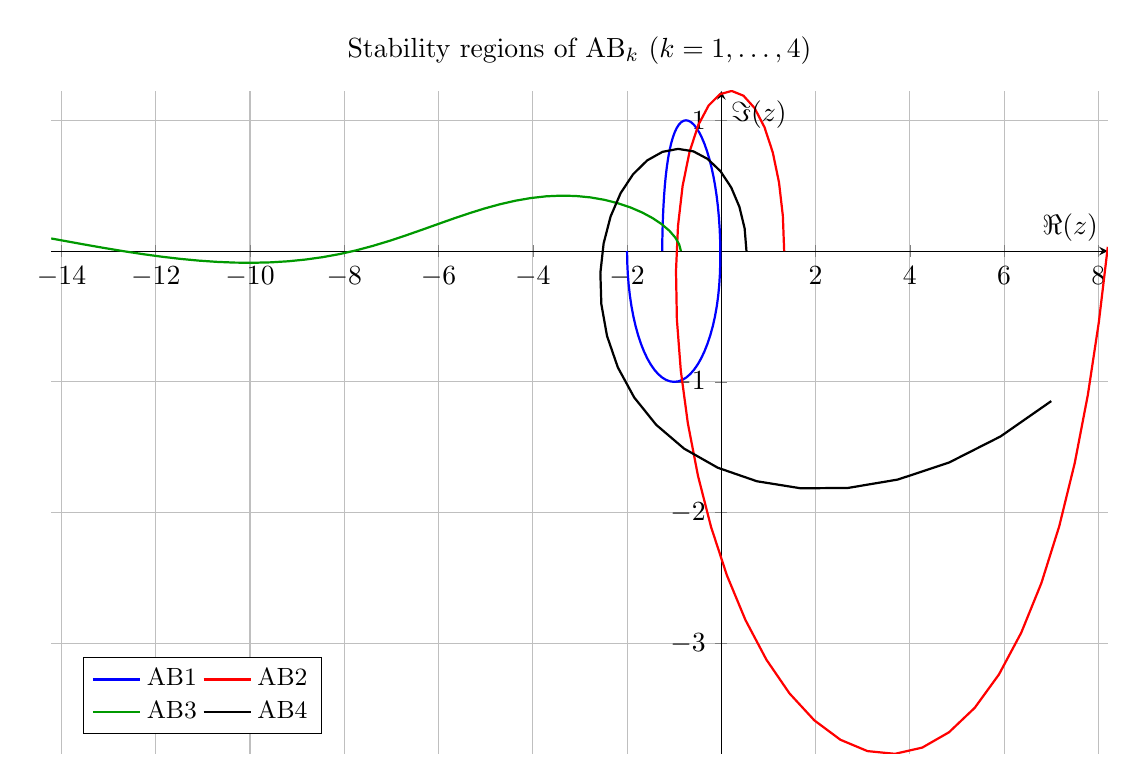
\begin{tikzpicture}
    \pgfplotstableread[col sep=space]{
        x y
        -2.000000 0.000000
        -1.996195 -0.087156
        -1.984808 -0.173648
        -1.965926 -0.258819
        -1.939693 -0.342020
        -1.906308 -0.422618
        -1.866025 -0.500000
        -1.819152 -0.573576
        -1.766044 -0.642788
        -1.707107 -0.707107
        -1.642788 -0.766044
        -1.573576 -0.819152
        -1.500000 -0.866025
        -1.422618 -0.906308
        -1.342020 -0.939693
        -1.258819 -0.965926
        -1.173648 -0.984808
        -1.087156 -0.996195
        -1.000000 -1.000000
        -0.912844 -0.996195
        -0.826352 -0.984808
        -0.741181 -0.965926
        -0.657980 -0.939693
        -0.577382 -0.906308
        -0.500000 -0.866025
        -0.426424 -0.819152
        -0.357212 -0.766044
        -0.292893 -0.707107
        -0.233956 -0.642788
        -0.180848 -0.573576
        -0.134975 -0.500000
        -0.096692 -0.422618
        -0.066399 -0.342020
        -0.044410 -0.258819
        -0.030003 -0.173648
        -0.022596 -0.087156
        -0.021102 0.000000
        -0.025816 0.087156
        -0.036002 0.173648
        -0.051783 0.258819
        -0.073139 0.342020
        -0.099946 0.422618
        -0.132000 0.500000
        -0.168994 0.573576
        -0.210530 0.642788
        -0.256127 0.707107
        -0.305236 0.766044
        -0.357256 0.819152
        -0.411548 0.866025
        -0.467464 0.906308
        -0.524362 0.939693
        -0.581619 0.965926
        -0.638646 0.984808
        -0.694892 0.996195
        -0.749861 1.000000
        -0.803110 0.996195
        -0.854243 0.984808
        -0.902909 0.965926
        -0.948814 0.939693
        -0.991721 0.906308
        -1.031452 0.866025
        -1.067867 0.819152
        -1.100876 0.766044
        -1.130440 0.707107
        -1.156565 0.642788
        -1.179297 0.573576
        -1.198722 0.500000
        -1.214969 0.422618
        -1.228208 0.342020
        -1.238646 0.258819
        -1.246514 0.173648
        -1.252062 0.087156
        -1.255554 0.000000
    }\ABone
    \pgfplotstableread[col sep=space]{
        x y
        1.333333 0.000000
        1.305215 0.269595
        1.223522 0.525322
        1.091548 0.754621
        0.915815 0.947181
        0.704815 1.094160
        0.468785 1.188406
        0.219422 1.224650
        -0.031210 1.199647
        -0.271276 1.112303
        -0.489401 0.963682
        -0.675904 0.756985
        -0.821915 0.497464
        -0.919515 0.192307
        -0.961840 -0.150931
        -0.943138 -0.523204
        -0.859830 -0.915055
        -0.710481 -1.316643
        -0.495798 -1.717930
        -0.218595 -2.108882
        0.118313 -2.479702
        0.511608 -2.821056
        0.956278 -3.124383
        1.445831 -3.382178
        1.972501 -3.588254
        2.527481 -3.737000
        3.101153 -3.823631
        3.683331 -3.844386
        4.263554 -3.796688
        4.831355 -3.679314
        5.376583 -3.492471
        5.889692 -3.237801
        6.362967 -2.918355
        6.790731 -2.538534
        7.169456 -2.104005
        7.497827 -1.621581
        7.776710 -1.099047
        8.009036 -0.544974
        8.199609 0.032562
    }\ABtwo
    \pgfplotstableread[col sep=space]{
        x y
        -0.857143 0.000000
        -0.895550 0.051861
        -0.978127 0.104018
        -1.102132 0.155497
        -1.263456 0.205267
        -1.457803 0.252261
        -1.680813 0.295417
        -1.928188 0.333708
        -2.195830 0.366185
        -2.479921 0.392026
        -2.777011 0.410564
        -3.084086 0.421330
        -3.398596 0.424075
        -3.718474 0.418786
        -4.042143 0.405694
        -4.368493 0.385283
        -4.696836 0.358255
        -5.026849 0.325529
        -5.358491 0.288198
        -5.691901 0.247487
        -6.027360 0.204707
        -6.365216 0.161211
        -6.705841 0.118335
        -7.049603 0.077359
        -7.396847 0.039456
        -7.747868 0.005663
        -8.102895 -0.023019
        -8.462083 -0.046514
        -8.825498 -0.064815
        -9.193128 -0.077974
        -9.564893 -0.086105
        -9.940633 -0.089387
        -10.320112 -0.088058
        -10.703021 -0.082407
        -11.088978 -0.072770
        -11.477534 -0.059526
        -11.868174 -0.043090
        -12.260312 -0.023903
        -12.653286 -0.002432
        -13.046368 0.020893
        -13.438769 0.045546
        -13.829642 0.070967
        -14.218093 0.096591
    }\ABthree
    \pgfplotstableread[col sep=space]{
        x y
        0.533333 0.000000
        0.494266 0.173331
        0.383730 0.338056
        0.210158 0.486178
        -0.017206 0.610395
        -0.288732 0.704308
        -0.593145 0.762679
        -0.917825 0.781630
        -1.249071 0.758829
        -1.572494 0.693629
        -1.873425 0.587201
        -2.137255 0.442558
        -2.349708 0.264493
        -2.497071 0.059425
        -2.566460 -0.166632
        -2.546080 -0.405341
        -2.425464 -0.648968
        -2.195739 -0.889474
        -1.849861 -1.118643
        -1.382770 -1.328247
        -0.791597 -1.510191
        -0.075813 -1.656642
        0.754965 -1.760144
        1.682270 -1.813764
        2.685664 -1.811248
        3.742944 -1.747180
        4.830425 -1.617078
        5.923275 -1.417487
        7.000000 -1.147059
    }\ABfour
    \begin{axis}[
            width=15cm, height=10cm,
            xlabel={$\Re(z)$}, ylabel={$\Im(z)$},
            title={Stability regions of $\mathrm{AB}_k$ ($k=1,\dots,4$)},
            axis lines=middle,
            grid=major,
            legend pos=south west,
            legend style={font=\small},
            legend columns=2,
        ]
        \addplot+[mark=none, thick, color=blue] table {\ABone};
        \addlegendentry{AB1}
        \addplot+[mark=none, thick, color=red] table {\ABtwo};
        \addlegendentry{AB2}
        \addplot+[mark=none, thick, color=green!60!black] table {\ABthree};
        \addlegendentry{AB3}
        \addplot+[mark=none, thick, color=black] table {\ABfour};
        \addlegendentry{AB4}
    \end{axis}
\end{tikzpicture}
\end{document}